%; whizzy paragraph -pdf xpdf -latex ./whizzypdfptex.sh
%; whizzy-paragraph "^\\\\begin{frame}\\|\\\\emtext"
% latex beamer presentation.
% platex, latex-beamer でコンパイルすることを想定。 

%     Tokyo Debian Meeting resources
%     Copyright (C) 2012 Junichi Uekawa

%     This program is free software; you can redistribute it and/or modify
%     it under the terms of the GNU General Public License as published by
%     the Free Software Foundation; either version 2 of the License, or
%     (at your option) any later version.

%     This program is distributed in the hope that it will be useful,
%     but WITHOUT ANY WARRANTY; without even the implied warreanty of
%     MERCHANTABILITY or FITNESS FOR A PARTICULAR PURPOSE.  See the
%     GNU General Public License for more details.

%     You should have received a copy of the GNU General Public License
%     along with this program; if not, write to the Free Software
%     Foundation, Inc., 51 Franklin St, Fifth Floor, Boston, MA  02110-1301 USA

\documentclass[cjk,dvipdfmx,12pt]{beamer}
\usetheme{Tokyo}
\usepackage{monthlypresentation}

%  preview (shell-command (concat "evince " (replace-regexp-in-string "tex$" "pdf"(buffer-file-name)) "&")) 
%  presentation (shell-command (concat "xpdf -fullscreen " (replace-regexp-in-string "tex$" "pdf"(buffer-file-name)) "&"))
%  presentation (shell-command (concat "evince " (replace-regexp-in-string "tex$" "pdf"(buffer-file-name)) "&"))

%http://www.naney.org/diki/dk/hyperref.html
%日本語EUC系環境の時
\AtBeginDvi{\special{pdf:tounicode EUC-UCS2}}
%シフトJIS系環境の時
%\AtBeginDvi{\special{pdf:tounicode 90ms-RKSJ-UCS2}}

\title{東京エリアDebian勉強会}
\subtitle{第91回 2012年8月度}
\author{上川純一\\dancer@debian.org}
\date{2012年8月18日}
\logo{
\includegraphics[width=8cm]{image200607/openlogo-light.eps}}

\begin{document}

\frame{\titlepage{}}

\begin{frame}{設営準備にご協力ください。}
会場設営よろしくおねがいします。
\end{frame}

\begin{frame}{Agenda}
\begin{minipage}[t]{0.45\hsize}
  \begin{itemize}
  \item 注意事項
	\begin{itemize}
	 \item 飲食禁止
	 \item 宗教禁止
	 \item 営利活動禁止
	\end{itemize}
   \item 最近あったDebian関連のイベント報告
	\begin{itemize}
        \item 第90回 東京エリアDebian勉強会
	\end{itemize}
 \end{itemize}
\end{minipage} 
\begin{minipage}[t]{0.45\hsize}
 \begin{itemize}
  \item Debian Conference 2012参加報告
  \item 月刊Debhelper
  \item ソフト開発以外の簡単Debian contribution(ドラフト版!)
  \item DebianでのC++11開発環境
 \end{itemize}
\end{minipage}
\end{frame}

\section{事前課題}
\emtext{事前課題}
{\footnotesize
 %; whizzy-master ../debianmeetingresume201208.tex
% $B0J>e$N@_Dj$r$7$F$$$k$?$a!"$3$N%U%!%$%k$G(B M-x whizzytex $B$9$k$H!"(Bwhizzytex$B$,MxMQ$G$-$^$9!#(B
%

\begin{prework}{ $BF|HfLn(B $B7<(B }

19$B<~G/$K$A$J$s$G!"$H$$$&$3$H$G$b$J$$$,!"(B
$B:#G/$O(B Haskell $B$N%i%$%V%i%j$r8x3+$9$kM=Dj$J$N$G!"(B
$B<+J,$G%Q%C%1!<%8%s%0$7$F%a%s%F%J$K$J$j$?$$!#(B
$B$"$H(B Debian Haskell $B%A!<%`$K$b;22C$7$F$$$-$?$$!#(B

\end{prework}

\begin{prework}{ $B$J$+$*$1$$$9$1(B }

$BJQ$o$i$:;H$$B3$1$^$9!#(B
$B$G!"$A$g$C$H$:$D!"(BContribute$B$7$F$$$3$&$H;W$C$F$^$9!#(B
\end{prework}

\begin{prework}{ $BLnEg!!5.1Q(B }

$BJzIi!'(B
$B!V2f$,$"$"(BDebian$B$N!ANO!J$j$g$/(B)$B$O$"$"$"$"@$3&$$$$$$%$%A%$%$%$%$%$%$(B
 $B%$!*!*!*!*!W$H$+8@$($k$HAGE($+$b(B...$B!J!A(B $B$NItJ,$OE,Ev$K(B...)
 
$B$A$g$C$H$0$i$$B>$N?M$,$d$C$?;v$,$J$$$3$H(B1$B$D$G$b(BDebian$B%M%?$G=PMh$?$i$$$$$J(B...$B!VL>>u$7$,$?$$2?$+$N%O!<%I%&%'%"!W$G(BDebian$BF0$+$7$F$_$k$H$+$+$J(B...

\end{prework}

\begin{prework}{ $B%-%?%O%i(B }

$B=tHL$NET9g$GGQ;_$5$l$F$7$^$C$?!"(B
$B2q<R$N(Bdebian$B%5!<%P$rI|3h$5$;$?$$$G$9$M!#(B

\end{prework}

\begin{prework}{ dictoss($B?yK\!!E5=<(B) }

kfreebsd$B$r;H$C$F3Z$7$_$J$,$i!"(Bdeb$B$7$F$$$-$^$9!#(B
\end{prework}

\begin{prework}{ $B@P0f0lIW(B }

DebConf$B$rF|K\$G3+:E$G$-$k$J$i$P!"@'Hs<B8=$5$;$?$$!#(B
\end{prework}

}

\section{Debian Conference 2012参加報告}
\emtext{Debian Conference 2012参加報告}


\section{月刊Debhelper}
\emtext{月刊Debhelper}

\begin{frame}{今回のお題は!}

\begin{itemize}
\item dh\_makeshlibs
\item dh\_shlibdeps
\end{itemize} 

\end{frame}

\begin{frame}{今回のお題は!}

\begin{itemize}
\item dh\_makeshlibs
\item dh\_shlibdeps
\end{itemize} 

\begin{center}
\Large
俺にとっては、まさに魔窟!秘境!\\
(ズガーン!)
\end{center}

\end{frame}

\begin{frame}{地図を手に入れた! ピロ〜ン♪}

 共有ライブラリの構造と流儀、動的リンクの方法、オブジェクトファイルの構造、debパッケージの構造について。

\begin{enumerate}
\item John R.Levine著 榊原 一矢/ポジティブエッジ 訳,「Linkers \& Loaders」,
ISBN10 4274064379
\item 坂井 弘亮著,「リンカ・ローダ実践開発テクニック」,ISBN10 4789838072
\item 高林 哲ら著,「Binary Hacks」,ISBN10 4873112885
\item Junichi Uekawa著,「Debian Library Packaging guide」,\\
\url{http://www.netfort.gr.jp/~dancer/column/libpkg-guide/libpkg-guide.html}
\item man 5 deb もしくはwikipediaのdeb(ファイルフォーマット)
\end{enumerate}

\end{frame}

\begin{frame}{今回のコマンドはそもそも何の為に!?}

{
 \Large
 バイナリとバイナリに必要な共有ライブラリとの関係を適切に自動生成する為\\
(依存関係算出はそもそも人手では「もう、やっとられんわーっ」という量にすぐになる為...)
 }

\end{frame}

\begin{frame}[containsverbatim]{「依存関係地獄(Dependency Hell)」からの攻撃!}

まあ、aptitude showとかで見ればわかる気がします...

\begin{commandline}
$ aptitude show gnome-shell
...中略...
依存: gir1.2-atk-1.0, gir1.2-clutter-1.0 (>= 1.9.16), 
   gir1.2-cogl-1.0, 
     gir1.2-coglpango-1.0,...中略...
   gnome-bluetooth (>= 3.0.0), 
     libatk1.0-0 (>= 1.12.4), libc6 (>= 2.7), 
   libcairo-gobject2 (>= 1.10.0), 
     libcairo2 (>= 1.10.0), libcanberra0 (>= 0.2), 
     libclutter-1.0-0 (>= 1.10.0), 
   libcogl-pango0 (>= 1.7.4),
     libcogl9 (>= 1.7.4), libcroco3 (>= 0.6.2), 
   libdbus-1-3 (>= 1.0.2), 
...「依存」の行は「まだまだまだ」続くぜ...
\end{commandline}
%$

\begin{center}
\Large
...祖はまさに「地獄」の名にふさわしい...
\end{center}


\end{frame}

\begin{frame}[containsverbatim]{debian/controlファイル中のマクロ(その1)}

ソースパッケージに入ってるdebian/control見ると...

\begin{commandline}
$ apt-get source gnome-shell
$ cd gnome-shell-3.2.1
$ less debian/control
...中略...
Package: gnome-shell
Architecture: any
Depends: ${gir:Depends},
         gjs (>= 1.29.18),
         ${shlibs:Depends},
         ${misc:Depends},
...中略...
\end{commandline}

なんか、マクロっぽいものがいっぱい。dh\_shlibdepsは、この場合、
\$\{shlibs:Depends\}を置き換えて、将来構築するDEBIAN/control(debパッケージに入る制御情報っすね)を生成します。
\end{frame}

\begin{frame}[containsverbatim]{debian/controlファイル中のマクロ(その2)}

補足:dh\_shlibdepsは能力的には、
\begin{itemize}
\item \$\{shlibs:Depends\}
\item \$\{shlibs:Suggests\}
\item \$\{shlibs:Recommends\}
\item \$\{shlibs:Pre-Depends\}
\end{itemize}

を依存関係算出して書き換える事が可能。が、\$\{shlibs:Depends\}以外は、どう使うのか自分的にはまだわからず..

\end{frame}

\begin{frame}{dh\_shlibdepsの動作}

\begin{center}
\Large
 次のスライドからとりあえず追ってみます。
\end{center}

\end{frame}

\begin{frame}[containsverbatim]{召喚! objdump その1}
バイナリ/共有ライブラリが必要としている他の共有ライブラリの情報一覧
\begin{commandline}
$ objdump -p /bin/ls | fgrep -A5 'Dynamic Section:'
Dynamic Section:
  NEEDED               libselinux.so.1
  NEEDED               librt.so.1
  NEEDED               libacl.so.1
  NEEDED               libc.so.6
  INIT                 0x0000000000402298
$ objdump -p /lib/x86_64-linux-gnu/libglib-2.0.so.0  |
 fgrep -A5 'Dynamic Section:'
Dynamic Section:
  NEEDED               libpcre.so.3
  NEEDED               libpthread.so.0
  NEEDED               librt.so.1
  NEEDED               libc.so.6
  SONAME               libglib-2.0.so.0
  INIT                 0x000000000001ba40

\end{commandline}

\end{frame}

\begin{frame}{召喚! objdump その2}

キーワード:

\begin{description}
\item [NEEDED] この項目で指定されるSONAMEを持つライブラリが必要という意味
\item [SONAME] ローダがライブラリを探すときに使う共有ライブラリの名前。本当の名前(real name)というのも別であるからややこしい...
(細かいこというと、本当はsonameは、libc.so.6なら、'c'がsoname。lib+'soname'+'.so.'+
'バージョン番号'となる。が、ここでは大文字でSONAMEとすればこちらのキーワードの値を指すことにする)
\end{description}


\end{frame}

\begin{frame}[containsverbatim]{召喚! objdump その3}

ライブラリの中の何が必要か?を表示してみる。

\begin{commandline}
$ objdump -T /bin/ls 
   ...中略...
DYNAMIC SYMBOL TABLE:
...中略... GLIBC_2.3   __ctype_toupper_loc
...中略... GLIBC_2.2.5 getenv
...中略... GLIBC_2.2.5 sigprocmask
...中略... GLIBC_2.2.5 raise
   ...中略...
$
\end{commandline}

(ちょっと、行長くてプレゼン資料に入りきらんので、各行の頭の部分は「...中略...」とさせてもらってます)

\end{frame}

\begin{frame}{召喚! shlibsファイル その1}

 すぐ思いつく(かもしれない)発想:\\
とりあえず、objdump -pの結果のNEEDEDのSONAMEから直接依存関係起こしちゃえば
いいんじゃね??

\end{frame}

\begin{frame}[containsverbatim]{召喚! shlibsファイル その2}

で、shlibsファイルが作られた。

\begin{commandline}
$ dpkg-query --control-path libgtk2.0-0
/var/lib/dpkg/info/libgtk2.0-0:amd64.shlibs
...中略...
$ cat /var/lib/dpkg/info/libgtk2.0-0:amd64.shlibs
libgtk-x11-2.0 0 libgtk2.0-0 (>= 2.24.0)
libgdk-x11-2.0 0 libgtk2.0-0 (>= 2.24.0)
udeb: libgtk-x11-2.0 0 libgtk2.0-0-udeb (>= 2.24.0)
udeb: libgdk-x11-2.0 0 libgtk2.0-0-udeb (>= 2.24.0)
\end{commandline}

意味は、例えばlibgtk-x11-2.0.so.0というSONAMEを見つけたら、依存情報として、
「libgtk2.0-0 ($>=$ 2.24.0)」と書け!という単純な構造。

(上の例の1行めの意味はlibgtk-x11-2.0+'.so.'+0 がSONAMEという意味)

\begin{center}
\Large
依存関係地獄は自動でやっつけれる!
\end{center}

\end{frame}

\begin{frame}[containsverbatim]{召喚! shlibsファイル その3}

 debian-policyマニュアルでは、
\begin{commandline}
$ git clone \
  http://anonscm.debian.org/git/dbnpolicy/policy.git
\end{commandline}
%$
するとshlibsについて定義が読めるよ!

\end{frame}

\begin{frame}{依存関係地獄復活! その1}

 一見よさそうにみえるshlibsを使った方法は実は以下の問題が...

\begin{itemize}
\item 実はこのshlibsに記載されている依存情報はパッケージ毎に固定のデータなので、ライブラリパッケージのバージョンが上がると、ライブラリに新たに追加されたシンボルを利用するバイナリの為に、依存情報にあるバージョンを上げざるを得ない。すると、新たに追加されたシンボルを使う必要の無いバイナリのパッケージは依存関係が満たせなくなってしまうのでインストール出来なくなる。
\end{itemize}

\end{frame}

\begin{frame}{依存関係地獄復活! その2}

\begin{itemize}
\item NEEDEDに記載されているSONAMEは、共有ライブラリのみが依存している他の共有ライブラリですら含んでしまっている。そのため、バイナリから見れば、直接リンクに関係無い共有ライブラリのバージョンが変わっても、パッケージはインストール出来なくなる。
\end{itemize}

 →このままでは、sid環境から、testing環境へバイナリパッケージだけを移動して動作させる事ができなくなっていく...

\end{frame}

\begin{frame}{依存関係地獄復活! その3}

 本当はこうなると良かった...
\begin{figure}[ht]
\begin{center}
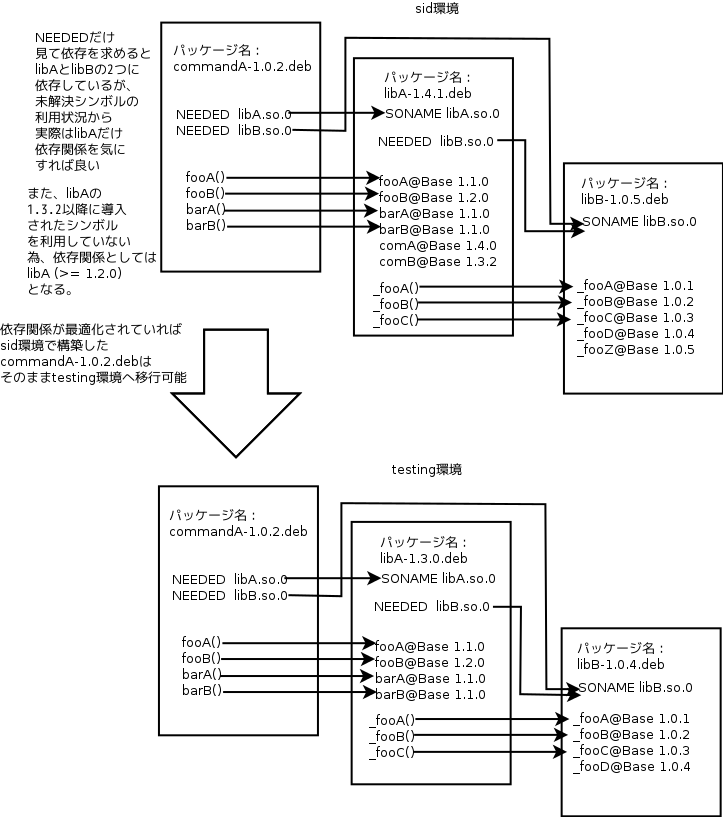
\includegraphics[scale=0.3]{image201208/symbols-advantage.png}
\end{center}
\end{figure}

\end{frame}

\begin{frame}{魔法使い(Wizard)現る! その1}

 Raphael(eはウムラウトね) Hertzogさんにより、
\begin{itemize}
\item shlibsファイルを使った依存関係の問題と解決の為の提案がなされる。\\
 Projects ImprovedDpkgShlibdeps\\
\url{http://wiki.debian.org/Projects/ImprovedDpkgShlibdeps}
\item 2007/9/25に、debian-devel-announceに、
この問題を解決する為の改造を施したdpkgコマンド群のリリースがアナウンスされた。\\
  New dpkg in experimental\\
 \url{http://lists.debian.org/debian-devel-announce/2007/09/msg00004.html}
\end{itemize}

\end{frame}

\begin{frame}{魔法使い(Wizard)現る! その2}

 参考:関係ないけど、Hertzogさんのblogサイトの名前は:\\
``apt-get install debian-wizard''\\
\url{http://raphaelherzog.com/}

 ...The DEBIAN ADMINISTRATOR'S HANDBOOKの著者ですね...

\end{frame}

\begin{frame}[containsverbatim]{召喚! symbolsファイル その1}

 さらに賢い依存関係を算出するために、symbolsファイルが導入された。

\begin{commandline}
$ dpkg-query --control-path libgtk2.0-0
...中略...
/var/lib/dpkg/info/libgtk2.0-0:amd64.symbols
...中略...
$ cat /var/lib/dpkg/info/libgtk2.0-0:amd64.symbols
libgdk-x11-2.0.so.0 libgtk2.0-0 #MINVER#
* Build-Depends-Package: libgtk2.0-dev
 gdk_add_client_message_filter@Base 2.8.0
 gdk_add_option_entries_libgtk_only@Base 2.8.0
 gdk_app_launch_context_get_type@Base 2.14.0
...中略...
\end{commandline}

 共有ライブラリのExportしているシンボルに、最初にシンボルが現れた時のdebパッケージバージョンがついている。

\end{frame}

\begin{frame}{召喚! symbolsファイル その2}

 前ページの例でいくと、バイナリに含まれるNEEDEDに、libgdk-x11-2.0.so.0が
入っていれば、依存情報として、''libgtk2.0-0 \#MINVER\#''を記載しなさいという意味。

 ここで、''\#MINVER\#''は、バイナリが必要とするシンボルが全部含まれるときのバージョンで置き換える。例えば、バイナリが gdk\_add\_client\_message\_filter, gdk\_add\_option\_entries\_libgtk\_only,gdk\_app\_launch\_context\_get\_typeのみを利用しているのであれば、''libgtk2.0-0 ( $>=$ 2.14.0 )''を依存関係として記載することになる。

\end{frame}

\begin{frame}{召喚! symbolsファイル その3}

 さらに、バイナリのNEEDEDに、libgtk2.0のみが利用している他のライブラリが
記載されていたとしても、バイナリの必要とするシンボルが含まれていなければ、
依存関係の候補として除外する。

 $\Longrightarrow$以上がdpkgコマンド群のdpkg-shlibdepsに実装された。\\
dh\_shlibdepsは新しい版のdpkg-shlibdepsをまるごとそっくり利用して依存関係を更新する。

\begin{center}
\Large
依存関係地獄は滅んだ!
\end{center}

\end{frame}

\begin{frame}{召喚! symbolsファイル その4}

 補足:このやり方だと、ライブラリのバージョンが上がってシンボルが廃止
になった場合は、自動で対応出来ないので、注意。

\end{frame}

\begin{frame}{dh\_makeshlibs}

 dh\_makeshlibsは、パッケージ構築ディレクトリにある構築完了した共有ライブラリからshlibsファイルを新規に生成し、同じようにsymbolsファイルをメンテナが用意したものから、新しいものへ更新するだけのdebhelperプログラムです。なお、symbolsファイルの更新に、dpkg-gensymbolsコマンドをそのまま用いています。

 なお、前ページで述べた問題を避ける為、dh\_makeshlibsは、symbolsファイルから、何かシンボルが消えた事を検知すると、エラー終了するように出来ています。(何が消えたかはdiff形式で標準出力に出力されます)
 
\begin{center}
\Large
dh\_makeshlibsの説明は以上っ
\end{center}

\end{frame}

\begin{frame}{次回}

\begin{center}
\Large
次回の発表者は...?
\end{center}

\end{frame}

\section{ソフト開発以外の簡単Debian contribution(ドラフト版!)}
\emtext{ソフト開発以外の簡単Debian contribution(ドラフト版!)}

\begin{frame}{ソフト開発以外の例 その1}

\begin{itemize}
\item DDTSSの日本語訳をレビューしてみる、日本語に訳してみる。\\
(詳しくは「第53回東京エリアDebian勉強会資料」\url{http://tokyodebian.alioth.debian.org/pdf/debianmeetingresume200906.pdf}を参照ください。非常に良い解説とチュートリアルとなっています。)
\item BTSへBUG報告/何かの改善提案をしてみる。\\
(詳しくは「第43回 関西Debian勉強会資料」\url{http://wiki.debian.org/KansaiDebianMeeting/20110123}を参照ください。非常に良い解説とチュートリアルとなっています。)
\end{itemize}

\end{frame}

\begin{frame}{ソフト開発以外の例 その2}
\begin{itemize}
\item \url{http://debtags.debian.net/edit/}でdebtagsをひたすら打ち込む。\\
(詳しくは「第63回東京エリアDebian勉強会資料」\url{http://tokyodebian.alioth.debian.org/pdf/debianmeetingresume201004.pdf}を参照ください。非常に良い解説とチュートリアルとなっています。)
\item \url{http://screenshots.debian.net/}へスクリーンショットを投稿しまくってみる。
\item \url{http://www.debianart.org/cchost/}へオリジナルの絵を送ってみる。
\item \url{debian-doc@debian.or.jp}にて投稿された翻訳のレビューをしてみる、未だ日本語に訳されていない文章を翻訳して投稿してみる。
\item \url{debian-users@debian.or.jp}にて投稿された質問に回答をしてみる。
\end{itemize}
\end{frame}

\begin{frame}{screenshots.debian.net その1}

\begin{itemize}
\item synapticパッケージでパッケージ調べて「screenshotsを見る」を押すと
screenshots.debian.netからスクリーンショットを落として表示します。
\item ユーザ登録もなしに、誰でもスクリーンショットを登録できます。(軽い審査はされますが...)
\end{itemize}

 使い方は、東京エリアDebian勉強会資料に記載しました。超簡単に投稿出来ます。

\end{frame}

\begin{frame}{screenshots.debian.net その2}

 自分もやってみた。

実例:
\begin{itemize}
\item renpy \\
\url{http://screenshots.debian.net/package/renpy}
\item renpy-demo \\
\url{http://screenshots.debian.net/package/renpy-demo}
\item zaz \\
\url{http://screenshots.debian.net/package/zaz}
\end{itemize}
等など...(実はゲームばっかりです)

\end{frame}

\begin{frame}{debianart.org}

\begin{itemize} 
\item   Debianに使われる様々なグラフィック/サウンドデータの投稿サイト。直近では、wheezyの起動画面の背景画像、GNOME環境のデフォルトの背景画像などのコンテストが行われた。
\item  最近では、Debianプロジェクトにマスコットキャラクタが必要ということで、マスコットキャラクタの図案の募集が行われていたようです。
\item デスクトップ用のファンファーレなどのサウンドアイコンもありました。
\end{itemize}

 絵心のある方/写真撮影に興味のある方/サウンドアイコンに興味ある方で、我こそはと
いう方はぜひ活用すると良いかもしれません。

\end{frame}

\begin{frame}{最後に}

 補足として、投稿したもの、提供したものは基本フリーなライセンスとなります。
ですので、以下は注意点となります。
 
\begin{itemize}
\item ライセンスで揉めそうなものは基本NGです。\\
例:有料ゲームのエミュレータのスクリーンショット、
ライセンスがよく分からない画像を利用などは避けるべきかと...
\end{itemize}

\end{frame}

\begin{frame}{ではネタだしを...}

\begin{center}
\Large
他にあったらぜひ教えて
\end{center}

\end{frame}

\section{DebianでのC++11開発環境}
\emtext{DebianでのC++11開発環境}

\begin{frame}{c++11}

\begin{itemize}
 \item 2011 年2月、ISO/IEC委員会にてC++11策定
 \item c++0xと呼ばれていた頃から各コンパイラーがドラフトを実装していたの
       で完全ではないが準拠している
 \item Debianで使ってみた
\end{itemize}
\end{frame}

\begin{frame}[containsverbatim]{wheezy での c++ コンパイラー}
\begin{itemize}
 \item g++ 4.7 \\ \url{http://gcc.gnu.org/projects/cxx0x.html}
 \item clang++ 3.0 \\
       \url{http://clang.llvm.org/cxx_status.html}
\end{itemize}
\begin{commandline}
# apt-get install g++ clang
\end{commandline}
\end{frame}

\begin{frame}[containsverbatim]{コードの例}
\begin{commandline}
#include <iostream>
using namespace std;

int main(int argc, char **argv) {
  int hoge[] = { 1, 10, 12, 15};
  const char* fuga[] = { "hello", "world", "this is a", "message"};
  for (const auto& i : hoge) {
    cout << i << endl;
  }

  for (const auto& str : fuga) {
    cout << str << endl;
  }
  return 0;
}
\end{commandline}
\end{frame}

\begin{frame}[containsverbatim]{コンパイルしてみる}
\begin{commandline}
$ g++ --std=c++11 auto.cc
$ clang++ --std=c++11 auto.cc 
\end{commandline}
\end{frame}

\begin{frame}{C++プログラミングするときにあると便利な参考文献}
\begin{itemize}
 \item stl-manual
 \item libstdc++6-4.7-doc
 \item gcc-doc
 \item libboost1.49-doc
 \item manpages-dev
 \item
      \url{http://www.open-std.org/jtc1/sc22/wg21/docs/papers/2011/n3242.pdf}
 \item \url{http://www.stroustrup.com/C++11FAQ.html}
\end{itemize}
\end{frame}

\begin{frame}{libc++}
 \begin{itemize}
  \item
       \url{http://wiki.debian.org/SummerOfCode2012/StudentApplications/AndrejBelym}
  \item libstdc++ switched to GPL3.
  \item C++11 
 \end{itemize}
\end{frame}
\end{document}

;;; Local Variables: ***
;;; outline-regexp: "\\([ 	]*\\\\\\(documentstyle\\|documentclass\\|emtext\\|section\\|begin{frame}\\)\\*?[ 	]*[[{]\\|[]+\\)" ***
;;; End: ***
